\documentclass[12pt,a4paper]{article}
\usepackage{graphicx} % Required for inserting images
\usepackage{tikz}
\usepackage[left=2.00cm, right=1.00cm]{geometry}
\usepackage{xcolor} % before tikz or tkz-euclide if necessary
\usepackage{amsmath}
\usepackage{siunitx}
\usepackage{chemfig}
\usetikzlibrary{calc}
\begin{document}
\begin{center}
    \large\textbf{prøve i termodynamikk:}
\end{center}
1.  Hvordan er temperaturskalaen Kelvin definert?\\\\
2.  Hva menes med det absolutte nullpunkt?\\\\
3. Hva sier den ideelle gasslov og hva er enhetene til de ulike verdiene?\\\\
4.  Regn om til Kelvin:  $35 ^\circ C, 63^\circ C, -26^\circ C, 253^\circ C $\\\\
5. Regn om til celisus: 273,15K, 233K, 57K, 800K\\\\
6. En gass innestengt i beholder har et trykk på $P_1=5,3bar$.  hvor stort blir trykket når vi halverer volumet og temperaturen er konstant? $V_1=6L$\\\\
7.  Vi har gitt følgende stempel med en gass som er innestengt.  Vi har et stempel som vi kan skyve inn og ut:\vspace{0.5cm}\\
\begin{center}
    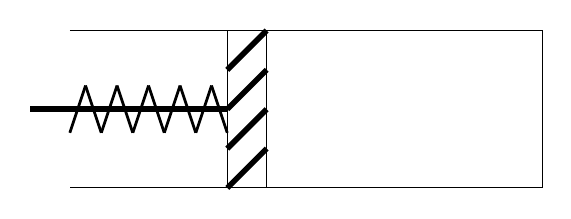
\begin{tikzpicture}
        %stempel med variabel
        \pgfmathsetmacro{\myLength}{4}
        \draw (2,2)--(8,2)--(8,0)--(2,0);
        \draw (\myLength,0)--(\myLength+0.5,0)--(\myLength+0.5,2)--(\myLength,2)--(\myLength,0);
        \draw [line width=2pt] (\myLength,0)--(\myLength+0.5,0.5);
        \draw [line width=2pt] (\myLength,0.5)--(\myLength+0.5,1);
        \draw [line width=2pt] (\myLength,1)--(\myLength+0.5,1.5);
        \draw [line width=2pt] (\myLength,1.5)--(\myLength+0.5,2);
        \draw [line width=2pt] (\myLength,1)--(\myLength-2.5,1);
        \draw [line width=1pt] (2,0.7)--(2.2,1.3);
        \draw [line width=1pt] (2.2,1.3)--(2.4,0.7);
        \draw [line width=1pt] (2.4,0.7)--(2.6,1.3);
        \draw [line width=1pt] (2.6,1.3)--(2.8,0.7);
        \draw [line width=1pt] (2.8,0.7)--(3.0,1.3);
        \draw [line width=1pt] (3.0,1.3)--(3.2,0.7);
        \draw [line width=1pt] (3.2,0.7)--(3.4,1.3);
        \draw [line width=1pt] (3.4,1.3)--(3.6,0.7);
        \draw [line width=1pt] (\myLength-0.4,0.7)--(\myLength-0.2,1.3);
        \draw [line width=1pt] (\myLength-0.2,1.3)--(\myLength,0.7);
    \end{tikzpicture}
\end{center}\vspace{1cm}
I starten er volumet $V_1=8L$ og trykket er lik $P_1=2,1bar$ .  Vi endrer volumet mens temperaturen er konstant slik at volumet blir $V_2=2L$.  Hva blir det nye trykket $P_2?$ \\\\
8.  Temperaturen til gassen er nå $T_2=52^\circ C$.  Vi øker temperaturen til $T_3=400K$.  Hva blir det nye trykket $P_3$ om vi antar at volumet er konstant?\newpage
Vi kan se på en firkantet kloss som ligger på et bord:\\\\\\\
\begin{center}
    \begin{tikzpicture}[scale=0.8]
        \draw (4,0)--(4,4);
        \draw (2,4)--(10,4);
        \draw (8,0)--(8,4);
        \draw (5,4) rectangle (7,6);
    \end{tikzpicture}    
\end{center}
Denne klossen har en masse 1,83kg og et areal som berører bordplaten.  Den yter dermedet trykk P mot bordet.  Sidene er lengde lik 30cm (0,3m), høyde lik 15cm (0,15m) og bredde lik 20cm (0,2m):\\
\begin{tikzpicture}[scale=1.5,transform canvas={shift={(6cm,-3cm)}}]


% Dimensjoner
\def\L{4}   % lengde
\def\B{2}   % bredde (dybde)
\def\H{1}   % høyde

% Vektor for dybde (perspektiv)
\coordinate (D) at (-0.5,0.3);

% Bunnflate
\draw (0,0) -- (\L,0) -- ++(D) -- ++(-\L,0) -- cycle;

% Vertikale kanter (høyde)
\draw (0,0) -- ++(0,\H);
\draw (\L,0) -- ++(0,\H);
\draw ($(0,0)+ (D)$) -- ++(0,\H);
\draw ($( \L,0) + (D)$) -- ++(0,\H);

% Toppflate
\draw (0,\H) -- (\L,\H) -- ++(D) -- ++(-\L,0) -- cycle;

% Linjer bakover (dybde)
\draw (\L,0) -- ++(D);
\draw (\L,\H) -- ++(D);
\node at (2,1.5) {lengde=30cm (0,3m)};
\node at (5.5,0.5) {høyde=15cm (0,15m)};
\node at (-1.8,0.2) {bredde=20cm (0,2m)};
\end{tikzpicture}\\
\vspace{4cm}
\\Denne klossen kan plasseres på tre forskjellig måter på bordet.  Beregn de tre ulike trykkene som klossen yter mot bordflaten.\\
Hint:
$$P=\frac{G}{A}$$
$G=m\cdot g$\\
G=tyngdekraften (N)\\
m=klossens masse (kg)\\
g=tyngdens akselerasjon ($m/s^2)$\\
P=trykket mot bordflaten $(N/m^2, Pa)$\\
A=Arealet til klossen mot bordplaten ($m^2$)\newpage
\noindent\large\textbf{Nyttige formler:}\\\\
Omregning mellom Kelvin og Celsius:\\
$T_K=T_C+273,15$\\
$T_C=T_K-273,15$\\\\
Den ideelle gasslov:\\\\
$P\cdot V=n\cdot R\cdot T$\\\\
Der:\\\\
P=gassens trykk (Pa, $N/m^2$)\\
n=antall molekyl, eller stoffmengde (mol)\\
R=gasskonstanten (8,314J/molK)\\
V=gassens volum ($m^3)$\\
T=temperaturen i K (kelvin)\newpage
\noindent\large\textbf{Gasslovene:}\\\\
\textbf{Ved konstant temperatur:}\\\\
$$P_1\cdot V_1=P_2\cdot V_2$$
P=trykk (bar eller Pa)\\
V=volum (mL eller L)\\\\
\textbf{"Kryss" for formelen:}\vspace{1cm}
\begin{center}
    \begin{tikzpicture}
        \draw (0,0) -- (4,0);
        \draw (2,-2) -- (2,2);
        \node at (4.4,0) {$V_1$};
        \node at (-0.4,0) {$P_1$};
        \node at (2,2.4) {$P_2$};
        \node at (2.1,-2.4) {$V_2$};
    \end{tikzpicture}
\end{center}
\textbf{Ved konstant trykk:}\\\\
$$\frac{V_1}{T_1}=\frac{V_2}{T_2}$$\\
T=tmeperatur(NB! MÅ være Kelvin)\\
V=volum (mL eller L)\newpage
\textbf{"Kryss" for formelen:}\vspace{1cm}
\begin{center}
    \begin{tikzpicture}
        \draw (0,0) -- (4,0);
        \draw (2,-2) -- (2,2);
        \node at (4.4,0) {$T_2$};
        \node at (-0.4,0) {$V_1$};
        \node at (2,2.4) {$V_2$};
        \node at (2.1,-2.4) {$T_1$};
    \end{tikzpicture}
\end{center}
\textbf{Ved konstant volum:}\\\\
$$\frac{P_1}{T_1}=\frac{P_2}{T_2}$$\\
P=trykk (bar eller Pa)\\
V=volum (mL eller L)\\\\
\textbf{"Kryss" for formelen:}\vspace{1cm}
\begin{center}
    \begin{tikzpicture}
        \draw (0,0) -- (4,0);
        \draw (2,-2) -- (2,2);
        \node at (4.4,0) {$T_2$};
        \node at (-0.4,0) {$P_1$};
        \node at (2,2.4) {$P_2$};
        \node at (2.1,-2.4) {$T_1$};
    \end{tikzpicture}
\end{center}

\end{document}